\section{Acerca de la tesis de licenciatura}

  \begin{itemize}
    \item Cosas que hice en la tesis de licenciatura.
    \begin{itemize}
    	\item[-] Corrección del clima
    	\item[-] Familiarizarse con el dataset
    \end{itemize}
    \item Resultados a los que llegué.
    \item Nos movimos a otros disparos (MoP y ToTs)
  \end{itemize}
  
   
  \begin{figure}[htbp]
    \centering
    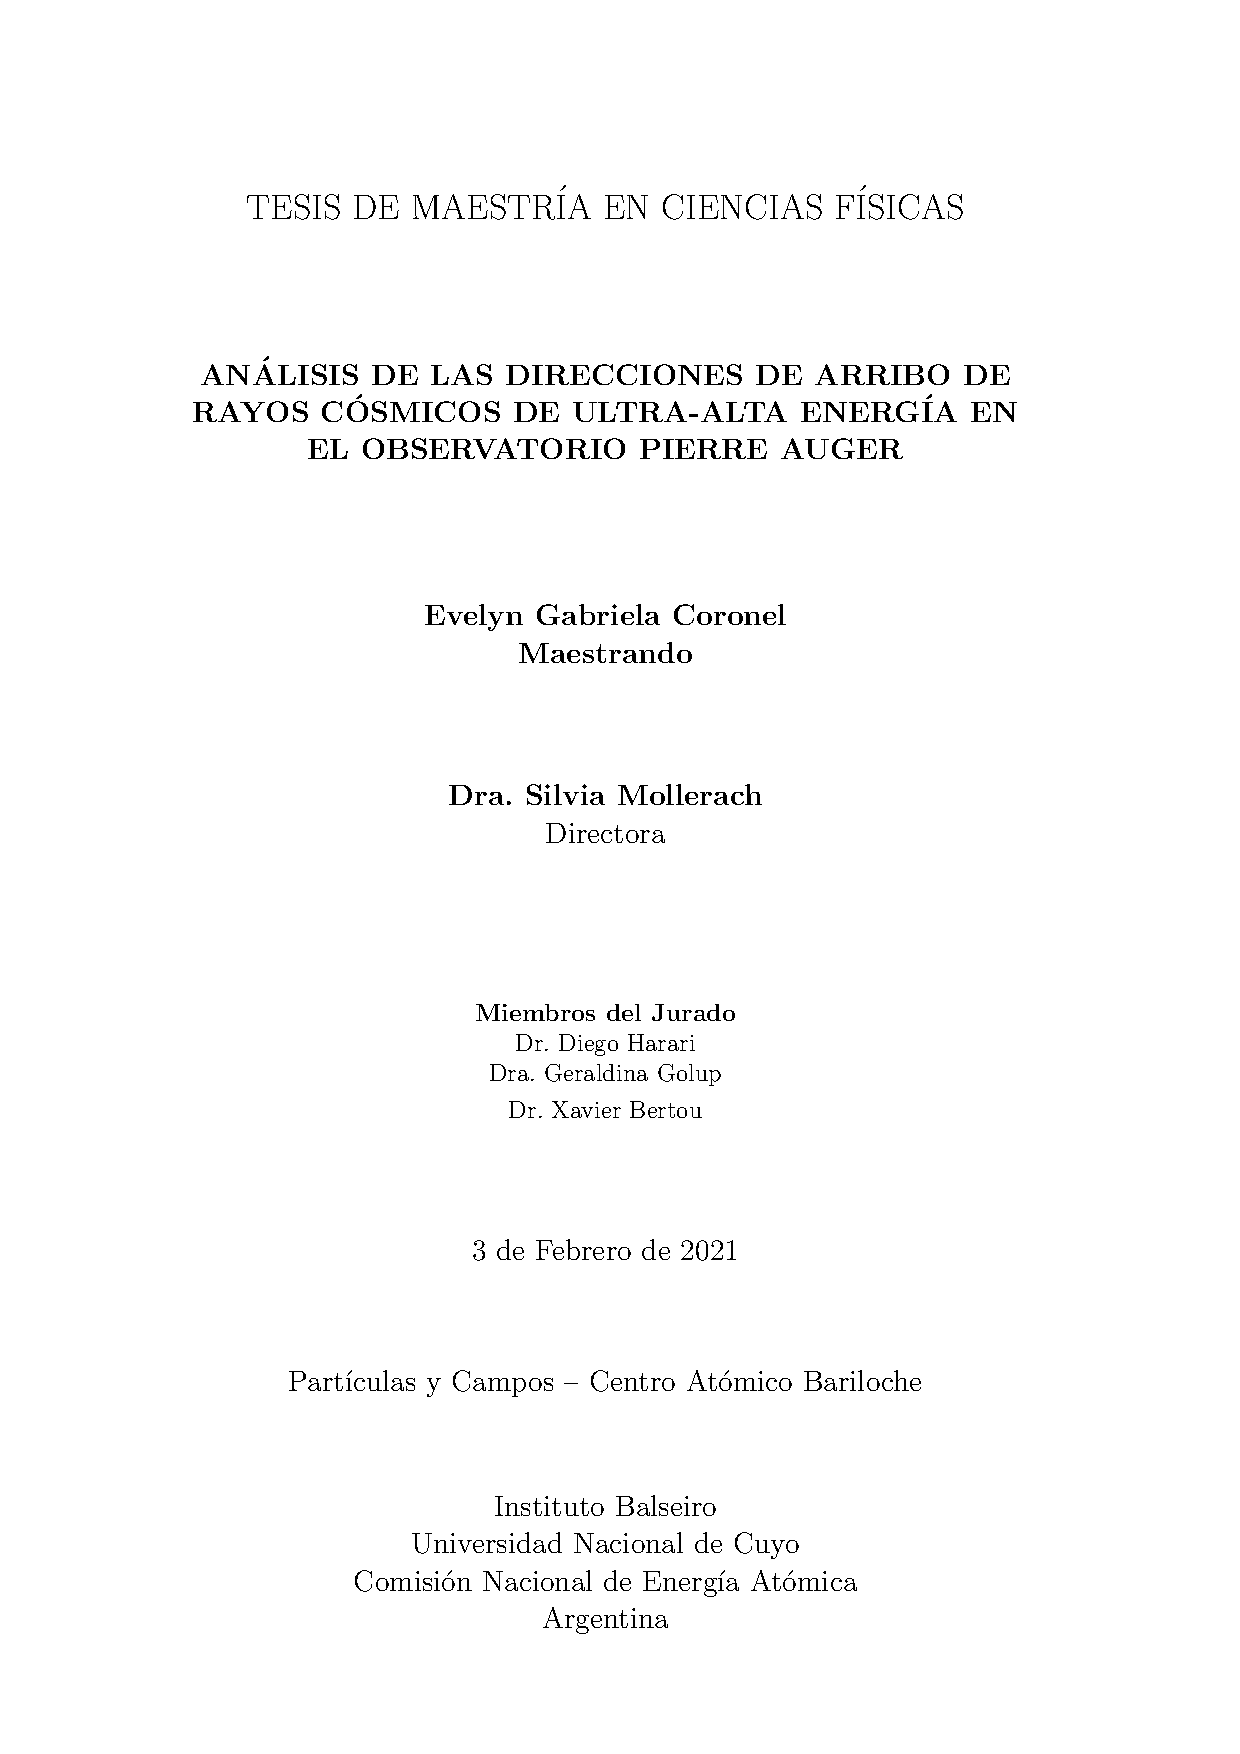
\includegraphics[width=0.95\textwidth]{../beamer-07-05-2020/tesis.png}
  \end{figure}
  
\section{Acerca del archivo con todos los disparos}

  \begin{itemize}
  	\item Diferencias con el disparo tradicional.
    \begin{itemize}
      \item[-] Empieza en el 2013
      \item[-] Eficiencia
      \item[-] Cantidad de datos en el bin de 1 EeV - 2 EeV.
    \end{itemize}
  	\item Pesos de los hexágonos.
  	\item Resultados con el rango de energía 1 EeV - 2 EeV.
    \item ¿Podemos mejorarlo con la corrección del clima?
  \end{itemize}

\section{Cálculo de Rayleigh.}

  \subsubsection{Pesos de los hexágonos}

      \begin{enumerate}
        \item Fijo una frecuencia a estudiar.
        \item Me muevo en el dataset de hexagonos, a cada utc lo clasifico según:
        \begin{equation*}
          h = (\text{hora local })\times \nicefrac{\text{Frecuencia a estudiar}}{\text{Frecuencia Solar}}
        \end{equation*}
          \item El valor de h no es continuo, sino está divido en 288 segmentos entre 1 y 24
       \item Le asigno un peso al bin h:
        \begin{align*}
          \text{peso del bin h} &= \nicefrac{\text{Hexagonos que cayeron en el bin h}}{I}\\
          I &= \sum^{288}_h \nicefrac{\text{Hexagonos que cayeron en el bin h}}{288}
         \end{align*} 
      \end{enumerate}

      Un ejemplo de lo que se obtiene


        \begin{figure}[H]
          \centering
              \includegraphics[width=0.85\linewidth]{../report_2_27_04_2020/weigth2005-2019.png}
              \caption{Pesos de los hexágonos en el rango 2005-2019 para distintas frecuencias.}
        \end{figure}

      % \begin{figure}[H]
      %   \centering
      %   \includegraphics[width=0.5\linewidth]{../report_2_27_04_2020/weigth2005-2019.png}
      %   \caption{Un ejemplo de pesos de los hexágonos en el rango 2005-2019 para distintas frecuencias.}
      % \end{figure}

      % \begin{figure}[H]
      %   \centering
      %   \includegraphics[width=0.5\linewidth]{../../Plotting/weigth2014-2019_jan.png}
      %   \caption{Un ejemplo de pesos de los hexágonos en el rango Enero 2014- Enero 2019 para distintas frecuencias.}
      % \end{figure}

  \subsubsection{Cálculo de Rayleigh para una frecuencia dada}

      \begin{enumerate}
        \item Fijo una frecuencia a estudiar.
        \item Me muevo en el cielo con esa frecuencia (fase).
        \item Dado el utc del evento, lo clasifico según:
        \begin{equation*}
          h = (\text{hora local })\times \nicefrac{\text{Frecuencia a estudiar}}{\text{Frecuencia Solar}}
        \end{equation*}
          \item El valor de h no es continuo, sino está divido en 288 segmentos entre 1 y 24
       \item Le asigno un peso por evento:
        \begin{equation*}
          \text{peso del evento} = (\text{peso  de los hexágonos para el bin h})^{-1}
          \end{equation*} 
         \item Hago el análisis en frecuencias:
         \begin{align*}
             a &= \sum^{Eventos}_i \cos(2\pi \nicefrac{h}{24} + (RA -RA_{cenit}))\times \nicefrac{(\text{peso del evento})_i}{N}\\
             b &= \text{Lo mismo pero con seno}\qquad         N = \sum^{Eventos}_i \text{peso del evento}_i
         \end{align*}
      \end{enumerate}